% Options for packages loaded elsewhere
\PassOptionsToPackage{unicode}{hyperref}
\PassOptionsToPackage{hyphens}{url}
%
\documentclass[
  12pt,
]{article}
\usepackage{amsmath,amssymb}
\usepackage{lmodern}
\usepackage{iftex}
\ifPDFTeX
  \usepackage[T1]{fontenc}
  \usepackage[utf8]{inputenc}
  \usepackage{textcomp} % provide euro and other symbols
\else % if luatex or xetex
  \usepackage{unicode-math}
  \defaultfontfeatures{Scale=MatchLowercase}
  \defaultfontfeatures[\rmfamily]{Ligatures=TeX,Scale=1}
\fi
% Use upquote if available, for straight quotes in verbatim environments
\IfFileExists{upquote.sty}{\usepackage{upquote}}{}
\IfFileExists{microtype.sty}{% use microtype if available
  \usepackage[]{microtype}
  \UseMicrotypeSet[protrusion]{basicmath} % disable protrusion for tt fonts
}{}
\makeatletter
\@ifundefined{KOMAClassName}{% if non-KOMA class
  \IfFileExists{parskip.sty}{%
    \usepackage{parskip}
  }{% else
    \setlength{\parindent}{0pt}
    \setlength{\parskip}{6pt plus 2pt minus 1pt}}
}{% if KOMA class
  \KOMAoptions{parskip=half}}
\makeatother
\usepackage{xcolor}
\usepackage[margin=1in]{geometry}
\usepackage{color}
\usepackage{fancyvrb}
\newcommand{\VerbBar}{|}
\newcommand{\VERB}{\Verb[commandchars=\\\{\}]}
\DefineVerbatimEnvironment{Highlighting}{Verbatim}{commandchars=\\\{\}}
% Add ',fontsize=\small' for more characters per line
\usepackage{framed}
\definecolor{shadecolor}{RGB}{248,248,248}
\newenvironment{Shaded}{\begin{snugshade}}{\end{snugshade}}
\newcommand{\AlertTok}[1]{\textcolor[rgb]{0.94,0.16,0.16}{#1}}
\newcommand{\AnnotationTok}[1]{\textcolor[rgb]{0.56,0.35,0.01}{\textbf{\textit{#1}}}}
\newcommand{\AttributeTok}[1]{\textcolor[rgb]{0.77,0.63,0.00}{#1}}
\newcommand{\BaseNTok}[1]{\textcolor[rgb]{0.00,0.00,0.81}{#1}}
\newcommand{\BuiltInTok}[1]{#1}
\newcommand{\CharTok}[1]{\textcolor[rgb]{0.31,0.60,0.02}{#1}}
\newcommand{\CommentTok}[1]{\textcolor[rgb]{0.56,0.35,0.01}{\textit{#1}}}
\newcommand{\CommentVarTok}[1]{\textcolor[rgb]{0.56,0.35,0.01}{\textbf{\textit{#1}}}}
\newcommand{\ConstantTok}[1]{\textcolor[rgb]{0.00,0.00,0.00}{#1}}
\newcommand{\ControlFlowTok}[1]{\textcolor[rgb]{0.13,0.29,0.53}{\textbf{#1}}}
\newcommand{\DataTypeTok}[1]{\textcolor[rgb]{0.13,0.29,0.53}{#1}}
\newcommand{\DecValTok}[1]{\textcolor[rgb]{0.00,0.00,0.81}{#1}}
\newcommand{\DocumentationTok}[1]{\textcolor[rgb]{0.56,0.35,0.01}{\textbf{\textit{#1}}}}
\newcommand{\ErrorTok}[1]{\textcolor[rgb]{0.64,0.00,0.00}{\textbf{#1}}}
\newcommand{\ExtensionTok}[1]{#1}
\newcommand{\FloatTok}[1]{\textcolor[rgb]{0.00,0.00,0.81}{#1}}
\newcommand{\FunctionTok}[1]{\textcolor[rgb]{0.00,0.00,0.00}{#1}}
\newcommand{\ImportTok}[1]{#1}
\newcommand{\InformationTok}[1]{\textcolor[rgb]{0.56,0.35,0.01}{\textbf{\textit{#1}}}}
\newcommand{\KeywordTok}[1]{\textcolor[rgb]{0.13,0.29,0.53}{\textbf{#1}}}
\newcommand{\NormalTok}[1]{#1}
\newcommand{\OperatorTok}[1]{\textcolor[rgb]{0.81,0.36,0.00}{\textbf{#1}}}
\newcommand{\OtherTok}[1]{\textcolor[rgb]{0.56,0.35,0.01}{#1}}
\newcommand{\PreprocessorTok}[1]{\textcolor[rgb]{0.56,0.35,0.01}{\textit{#1}}}
\newcommand{\RegionMarkerTok}[1]{#1}
\newcommand{\SpecialCharTok}[1]{\textcolor[rgb]{0.00,0.00,0.00}{#1}}
\newcommand{\SpecialStringTok}[1]{\textcolor[rgb]{0.31,0.60,0.02}{#1}}
\newcommand{\StringTok}[1]{\textcolor[rgb]{0.31,0.60,0.02}{#1}}
\newcommand{\VariableTok}[1]{\textcolor[rgb]{0.00,0.00,0.00}{#1}}
\newcommand{\VerbatimStringTok}[1]{\textcolor[rgb]{0.31,0.60,0.02}{#1}}
\newcommand{\WarningTok}[1]{\textcolor[rgb]{0.56,0.35,0.01}{\textbf{\textit{#1}}}}
\usepackage{graphicx}
\makeatletter
\def\maxwidth{\ifdim\Gin@nat@width>\linewidth\linewidth\else\Gin@nat@width\fi}
\def\maxheight{\ifdim\Gin@nat@height>\textheight\textheight\else\Gin@nat@height\fi}
\makeatother
% Scale images if necessary, so that they will not overflow the page
% margins by default, and it is still possible to overwrite the defaults
% using explicit options in \includegraphics[width, height, ...]{}
\setkeys{Gin}{width=\maxwidth,height=\maxheight,keepaspectratio}
% Set default figure placement to htbp
\makeatletter
\def\fps@figure{htbp}
\makeatother
\setlength{\emergencystretch}{3em} % prevent overfull lines
\providecommand{\tightlist}{%
  \setlength{\itemsep}{0pt}\setlength{\parskip}{0pt}}
\setcounter{secnumdepth}{-\maxdimen} % remove section numbering
\usepackage{xcolor}
\usepackage{hyperref}
\usepackage{pdfcomment}
\usepackage{fancyhdr} \pagestyle{fancy} \setlength{\headheight}{75pt} \setlength{\textheight}{600pt} \fancyhead[C]{} \fancyhead[L]{
\includegraphics{X:/DSA/shiny-uploads/images/PST_Equity_Edition-Trend_header.png}} \fancyhead[R]{} \fancyfoot[L]{\scriptsize{1011 Western Ave, Suite 500, Seattle WA 98104} \textcolor[HTML]{F05A28}. 206.464.7532 \textcolor[HTML]{F05A28}. www.psrc.org \textcolor[HTML]{F05A28}. February 2023} \fancyfoot[R]{\textcolor[HTML]{F05A28}\thepage} \fancyfoot[C]{} \renewcommand{\headrulewidth}{0pt} \renewcommand{\footrulewidth}{4pt} \renewcommand{\footrule}{\hbox to \headwidth{\color[HTML]{BCBEC0}\leaders\hrule height \footrulewidth\hfill}}
\usepackage{fontspec}\fancyhead[C]\fancyhead[L]{
\includegraphics{X:/DSA/shiny-uploads/images/PST_Equity_Edition-Trend_header.png}}
\ifLuaTeX
  \usepackage{selnolig}  % disable illegal ligatures
\fi
\IfFileExists{bookmark.sty}{\usepackage{bookmark}}{\usepackage{hyperref}}
\IfFileExists{xurl.sty}{\usepackage{xurl}}{} % add URL line breaks if available
\urlstyle{same} % disable monospaced font for URLs
\hypersetup{
  pdfauthor={Suzanne Childress \& Meg Grzybowski},
  hidelinks,
  pdfcreator={LaTeX via pandoc}}

\author{Suzanne Childress \& Meg Grzybowski}
\date{2023-02-16}

\begin{document}

\setmainfont{Poppins}

\hypertarget{understanding-womens-travel-for-womens-history-month}{%
\section{Understanding Women's Travel for Women's History
Month}\label{understanding-womens-travel-for-womens-history-month}}

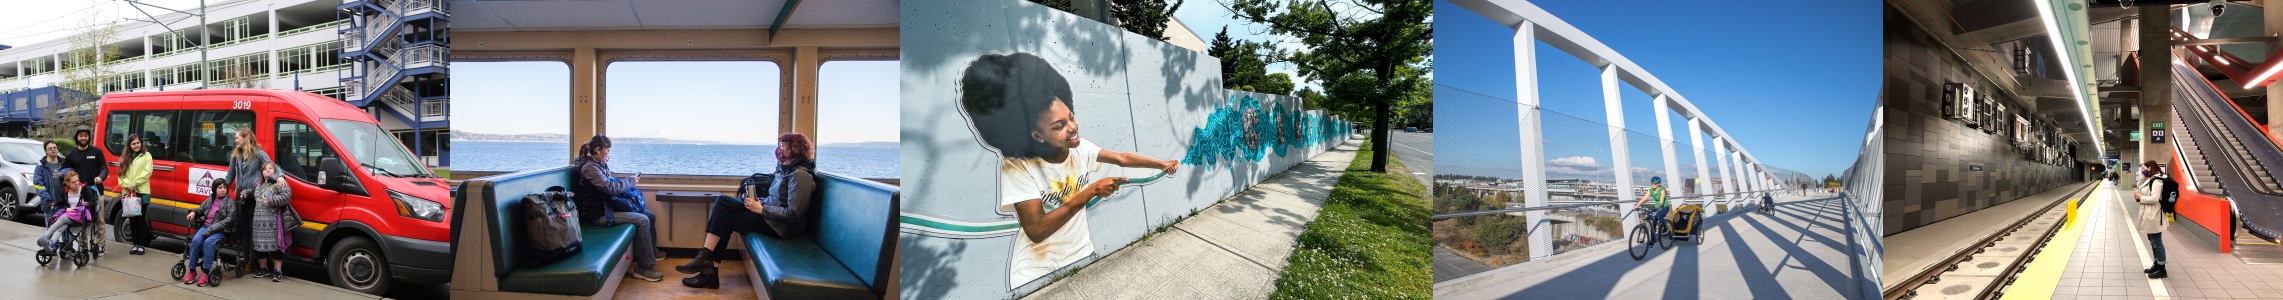
\includegraphics[width=1\textwidth,height=\textheight]{C:/Coding/CURRENT_REPOS_GITHUB/document-maker/templates/equity_example/women2_image_header.png}

\textbackslash begin\{document\} Women have
\href{http://libraryarchives.metro.net/DB_Attachments/2019-0294/UnderstandingHowWomenTravel_FullReport_FINAL.pdf}{\underline{\textcolor{blue}{transportation needs that have not historically been met}}}.
The regional transportation system, including transit, was designed
around the need to quickly get to work at central locations. Women carry
significantly more of the care-giving burden's of society and thus need
a system that works safely for traveling with others to a variety of
locations at all times of day. Women also represent a large portion of
older populations who have unique transportation needs, not well-served
by our system built for driving and going to work locations. Women are
also more likely to live in poverty and have lower incomes than men.

As the world evolves post-COVID towards greater telecommuting for some
people and continued trends in aging, will the transportation system
evolve for women?

\hypertarget{household-travel-survey}{%
\paragraph{Household Travel Survey}\label{household-travel-survey}}

The 2017, 2019, and 2021 household travel surveys collected day-to-day
information from households in the central Puget Sound region, such as
how we traveled, where we went, how long it took---even where we chose
to live and whether we got home deliveries, prior to COVID-19 and after.

This report starts with comparison of travel by gender, during the
stable period prior to COVID-19, and then dives into some recent trends
that occured in 2021, during COVId-19. Learn more at the
\href{https://www.psrc.org/our-work/household-travel-survey-program}{\underline{\textcolor{blue}{household travel survey webpage}}}.Data
from 2017 and 2019 have combined to give a more robust sample size. You
can also
\href{https://household-travel-survey-psregcncl.hub.arcgis.com}{\underline{\textcolor{blue}{view the full survey dataset here}}},
including 2017, 2019 and 2021 data.

notes: Fewer women work than men. Women take few work trips, more
caregiving related trips, more household chore trips.The transit system
was initially designed around traveling to a central city work location-
which may not meet women's needs as well as men's (on average).Women
live longer than men, so that at older ages there are many more women
who have unique travel needs than men.Older people (who tend to be women
more often) have more need for transit in off-peak hours and specialized
transportation services.Women bike much less than men. Some of this is
undoubtedly because of bike network design not being safe for all
people.How can the transportation and land use system better accommodate
older people, household maintenance and caregiving needs? Addressing
these questions will improve the system for all genders.

start with 2017/2019 data; transition to pandemic data?

according to 2021 hhts, 103, 000 women live in a household without a
car; 86,000 men

from:

Travel Behavior Trends Through the analysis in this report, key trends
emerge that differentiate women's travel patterns from men's travel
patterns, across all modes. » Across all modes, more women are making
many trips (7 or more) per day than men and more women than men are not
making any trips per day. This means women may experience more exposure
to travel burdens (cost, stress, or safety risks), or may be more likely
to be isolated or disconnected from the opportunities that travel
affords. » Women in Los Angeles also make shorter trips than men, which
is potentially driven by workforce participation rates, location of
employment opportunities, and taking household-serving trips that tend
to be more localized. » Women's trips are more varied to a broader
spread of destinations, and are more likely to primarily serve the needs
of someone else. » Women are more likely to live in a car-free or
carlight household, take more trips with other people, and take fewer
single-occupant car trips than men. » Women are also more likely to
carpool or get a ride from a family member or friend if they don't have
a driver's license. These findings show that women may need to adjust
their own schedule and travel needs to accommodate others, and in doing
so, give up some of their own autonomy and control over when and how
they travel. Despite these challenges and tradeoffs, women show
ingenuity in arranging their schedules to meet their travel needs. »
Women are more likely to trip-chain, or make stops along the way to
other destinations, and describe consolidating all their errand trips
into one day where they will have access to a vehicle. » Women in Los
Angeles are also more likely than men to travel mid-day, with a travel
peak around 2 PM when transit service may be reduced.

Among female riders, almost 90\% ride the system more than three days
per week. » 57\% of women bring their children on transit. » Women ride
transit because they do not have a car, because they want to avoid
traffic, or because they do not have a license. Two of these three
reasons indicate that women who ride transit do so because they have
fewer transportation options, and may have less access to economic
opportunities as a result. Still, many women do use transit to access
economic opportunity. » Over 85\% of women riders use Metro to travel to
work or school, and of those women, 32\% also use Metro to run errands
or complete recreational trips. Among people who make household serving
trips most frequently, these trips comprise the same share for women
whether they use transit or not; for men, the share of household-serving
trips declines if they are transit users. This shows that while men are
more likely to find alternatives to using transit to complete
household-serving trips (using a different mode or taking fewer trips),
women are less likely to find an alternative, and instead work to make
the transit system work for their needs. Although the rate of adoption
for TNCs like Uber and Lyft is the same for men and women, women are
more likely than men to report that their transit use has stayed the
same as they have also begun to use TNCs. » Women are more likely than
men to say they use TNCs for trips that transit does not serve, while
men are more likely to say they use TNCs to reach a transit stop or
station. The trips that are not served by transit may be related to time
or location, as women's needs differ from men's needs by both time of
day and location. These travel behavior findings point towards many
opportunities to adjust the services provided by Metro to better meet
the travel needs expressed by those who are using transit. Development
of a Gender Action Plan - or a tactical plan to implement policy,
design, and service changes throughout the agency - would help to
articulate the immediate opportunities and long-term goals that would
create a system that better serves women. Adjustments to services,
vehicle design, and policy would help minimize the time, cost, safety,
and physical burdens of riding transit for the more than half of all
riders who are women. » The findings from Understanding How Women Travel
about women's mode choices, how likely they are to travel with others in
their care, and their complex trip-chaining patterns could all inform
adjustments to Metro's fare policy to make it more equitable towards
women and more cost-competitive with driving and carpooling. »Findings
about women's trip purposes and primary responsibility for household
errands could all inform the way transit vehicles, transit stations, and
bus stops are designed, so that space for traveling with others and
carrying bags and other belongings could be better accommodated.
»Findings about when women are traveling and average trip lengths could
inform new service offerings that meet a mid-day peak travel demand and
provide better direct connections over long distances while minimizing
transfers.

Vehicle access issues disproportionately affect women.

Financial access also disproportionately affects women. Low-income
women, in particular, carry a disproportiona

\hypertarget{some-header}{%
\subsection{some header}\label{some-header}}

Women make more trips for care-giving purposes like escort passengers,
shopping, household errands, and less trips for work and school. The
transportation system is set up for people to get quickly to work.

Note to Megan: add axis titles
\includegraphics{womens_history_story_draft_files/figure-latex/unnamed-chunk-2-1.pdf}
PUMS data shows women are employed more than men, but not to the extent
the trip purposes diverge. Women who are working are still carrying more
burden of other household tasks.

\begin{Shaded}
\begin{Highlighting}[]
\NormalTok{pums\_19\_all\_employed}\OtherTok{\textless{}{-}}\NormalTok{ pums19\_all }\SpecialCharTok{\%\textgreater{}\%} \FunctionTok{filter}\NormalTok{(ESR}\SpecialCharTok{==}\StringTok{\textquotesingle{}Employed\textquotesingle{}}\NormalTok{) }


\NormalTok{employ\_\_gender\_chart\_19 }\OtherTok{\textless{}{-}} \FunctionTok{static\_column\_chart}\NormalTok{(}\AttributeTok{t=}\NormalTok{pums\_19\_all\_employed, }
                                    \AttributeTok{x =} \StringTok{"SEX"}\NormalTok{,}
                                    \AttributeTok{y =} \StringTok{"share"}\NormalTok{,}
                                    \AttributeTok{fill =} \StringTok{"SEX"}\NormalTok{,}
                                    \AttributeTok{color=}\StringTok{"psrc\_pairs"}\NormalTok{,}
                                    \AttributeTok{est =}\StringTok{"percent"}\NormalTok{,}
                                    \AttributeTok{title =} \StringTok{"2019 Employment by Gender"}\NormalTok{,}
                                    \AttributeTok{source =} \StringTok{"Source: American Community Survey 1019 1{-}year data Sex by Employment Status"}\NormalTok{)}

\NormalTok{employ\_\_gender\_chart\_19}
\end{Highlighting}
\end{Shaded}

\includegraphics{womens_history_story_draft_files/figure-latex/unnamed-chunk-3-1.pdf}
Women take shorter more local trips, as opposed to long highway trips.
The transportation system needs to be set up for people getting to a
variety of locations by a variety of modes.

\begin{Shaded}
\begin{Highlighting}[]
\FunctionTok{static\_column\_chart}\NormalTok{(}\AttributeTok{t=}\NormalTok{ summs\_2017\_2019\_dist, }\AttributeTok{x=}\StringTok{\textquotesingle{}gender\textquotesingle{}}\NormalTok{, }\AttributeTok{y=}\StringTok{\textquotesingle{}trip\_path\_distance\_median\textquotesingle{}}\NormalTok{,  }\AttributeTok{fill=}\StringTok{\textquotesingle{}gender\textquotesingle{}}\NormalTok{, }\AttributeTok{moe=}\StringTok{\textquotesingle{}trip\_path\_distance\_median\_moe\textquotesingle{}}\NormalTok{, }\AttributeTok{est=}\StringTok{\textquotesingle{}number\textquotesingle{}}\NormalTok{, }\AttributeTok{title=}\StringTok{\textquotesingle{} Trip Distance by Gender\textquotesingle{}}\NormalTok{, }\AttributeTok{source=} \StringTok{\textquotesingle{}Source: 2017/2019 Household Travel Survey\textquotesingle{}}\NormalTok{)}
\end{Highlighting}
\end{Shaded}

\includegraphics{womens_history_story_draft_files/figure-latex/unnamed-chunk-4-1.pdf}
Women in households with more than two people tend to travel more with
other people than men. Transit is often not well set up for people who
are traveling with strollers. The walk and bike network are not built
out for people of all ages to use.

\begin{Shaded}
\begin{Highlighting}[]
\FunctionTok{static\_column\_chart}\NormalTok{(}\AttributeTok{t=}\NormalTok{ trav\_summs\_2017\_2019, }\AttributeTok{x=}\StringTok{\textquotesingle{}travelers\_total\_grp\textquotesingle{}}\NormalTok{, }\AttributeTok{y=}\StringTok{\textquotesingle{}share\textquotesingle{}}\NormalTok{,  }\AttributeTok{fill=}\StringTok{\textquotesingle{}gender\textquotesingle{}}\NormalTok{, }\AttributeTok{moe=}\StringTok{\textquotesingle{}share\_moe\textquotesingle{}}\NormalTok{, }\AttributeTok{est=}\StringTok{\textquotesingle{}percent\textquotesingle{}}\NormalTok{, }\AttributeTok{title =} \StringTok{\textquotesingle{}Percent of Trips by Number of Travelers, for People in Households with more than 2 people\textquotesingle{}}\NormalTok{,  }\AttributeTok{source=} \StringTok{\textquotesingle{}Source: 2017/2019 Household Travel Survey\textquotesingle{}}\NormalTok{ )}
\end{Highlighting}
\end{Shaded}

\includegraphics{womens_history_story_draft_files/figure-latex/unnamed-chunk-5-1.pdf}
Women represent a greater share of the older population who needs more
specialized transportation services, and less service to work locations.
\url{https://www.nytimes.com/2022/12/03/health/elderly-living-alone.html}

\begin{Shaded}
\begin{Highlighting}[]
\FunctionTok{static\_column\_chart}\NormalTok{(pums19\_sex\_age, }\AttributeTok{x=} \StringTok{\textquotesingle{}BIN\_AGE\textquotesingle{}}\NormalTok{, }\AttributeTok{y=} \StringTok{\textquotesingle{}share\textquotesingle{}}\NormalTok{, }\AttributeTok{fill=} \StringTok{\textquotesingle{}SEX\textquotesingle{}}\NormalTok{, }\AttributeTok{source=}\StringTok{\textquotesingle{}Source: 2019 Public Use Microsample Census data\textquotesingle{}}\NormalTok{)}
\end{Highlighting}
\end{Shaded}

\includegraphics{womens_history_story_draft_files/figure-latex/unnamed-chunk-6-1.pdf}
THe bike network is not well-suited for women's needs because it feels
unsafe for people of different ages and abilities. As a result, in 2019
only 30,000 bike trips were made by women but 74,000 men.

\begin{Shaded}
\begin{Highlighting}[]
\FunctionTok{static\_column\_chart}\NormalTok{(}\AttributeTok{t=}\NormalTok{ mode\_summs\_2017\_2019, }\AttributeTok{x=}\StringTok{\textquotesingle{}mode\_simple\textquotesingle{}}\NormalTok{, }\AttributeTok{y=}\StringTok{\textquotesingle{}count\textquotesingle{}}\NormalTok{,  }\AttributeTok{fill=}\StringTok{\textquotesingle{}gender\textquotesingle{}}\NormalTok{, }\AttributeTok{est=}\StringTok{\textquotesingle{}number\textquotesingle{}}\NormalTok{, }\AttributeTok{source =} \StringTok{\textquotesingle{}Source: 2019 PSRC Household Travel Survey Data\textquotesingle{}}\NormalTok{)}
\end{Highlighting}
\end{Shaded}

\includegraphics{womens_history_story_draft_files/figure-latex/unnamed-chunk-7-1.pdf}
COVID-19 brought about abrupt changes to the transportation landscape.
The 2021 Household Travel survey showed big changes in travel behavior.
More people were walking and biking, and less people were using transit.
Many more people began to telework. Women teleworked more than men,
before COVID-19, and the data shows this difference increase even more
in 2021. In 2021, 41\% of women teleworked, as compared to 33\% of men.
The difference between telework rates relates to women's job sectors as
compared to men, and also household responsibilities.

Increase in telecommuting may be a double edged sword for women- still
have hh responsibilities; but also juggling work

\begin{Shaded}
\begin{Highlighting}[]
\FunctionTok{static\_line\_chart}\NormalTok{(}\AttributeTok{t=}\NormalTok{ work\_loc\_trend, }\AttributeTok{x=}\StringTok{\textquotesingle{}survey\textquotesingle{}}\NormalTok{, }\AttributeTok{y=}\StringTok{\textquotesingle{}share\textquotesingle{}}\NormalTok{,  }\AttributeTok{fill=}\StringTok{\textquotesingle{}gender\_group\textquotesingle{}}\NormalTok{, }\AttributeTok{est=}\StringTok{\textquotesingle{}percent\textquotesingle{}}\NormalTok{)}\SpecialCharTok{+}
                                \FunctionTok{xlab}\NormalTok{(}\StringTok{\textquotesingle{}Year\textquotesingle{}}\NormalTok{)}\SpecialCharTok{+}\FunctionTok{ylab}\NormalTok{(}\StringTok{\textquotesingle{}Percent of Workers\textquotesingle{}}\NormalTok{)}\SpecialCharTok{+}
                                \FunctionTok{scale\_x\_discrete}\NormalTok{()}
\end{Highlighting}
\end{Shaded}

\begin{verbatim}
## Scale for x is already present.
## Adding another scale for x, which will replace the existing scale.
\end{verbatim}

\includegraphics{womens_history_story_draft_files/figure-latex/unnamed-chunk-8-1.pdf}

In 2021, people were traveling for different purposes.

\begin{Shaded}
\begin{Highlighting}[]
\FunctionTok{static\_facet\_column\_chart}\NormalTok{(}\AttributeTok{t=}\NormalTok{ summs\_2017\_2019\_2021, }\AttributeTok{x=}\StringTok{\textquotesingle{}simple\_purpose\textquotesingle{}}\NormalTok{, }\AttributeTok{y=}\StringTok{\textquotesingle{}share\textquotesingle{}}\NormalTok{,  }\AttributeTok{fill=}\StringTok{\textquotesingle{}gender\textquotesingle{}}\NormalTok{, }\AttributeTok{facet=}\StringTok{\textquotesingle{}survey\textquotesingle{}}\NormalTok{, }\AttributeTok{moe=}\StringTok{\textquotesingle{}share\_moe\textquotesingle{}}\NormalTok{, }\AttributeTok{est=}\StringTok{\textquotesingle{}percent\textquotesingle{}}\NormalTok{)}
\end{Highlighting}
\end{Shaded}

\includegraphics{womens_history_story_draft_files/figure-latex/unnamed-chunk-9-1.pdf}
What else?

\subsection{Conclusion}

someotherwords

\fancyhead[L]{}

\end{document}
